\section{Park Generation}

Once the PlotGenerator is finished, the ParkGenerator, BuildingGenerator, and ParkingGenerator work in parallel to fill the generated plots with interesting content.
After all these generators have finished running the generated city may look something like this (see Figure~\ref{fig:ex}).
\begin{figure}
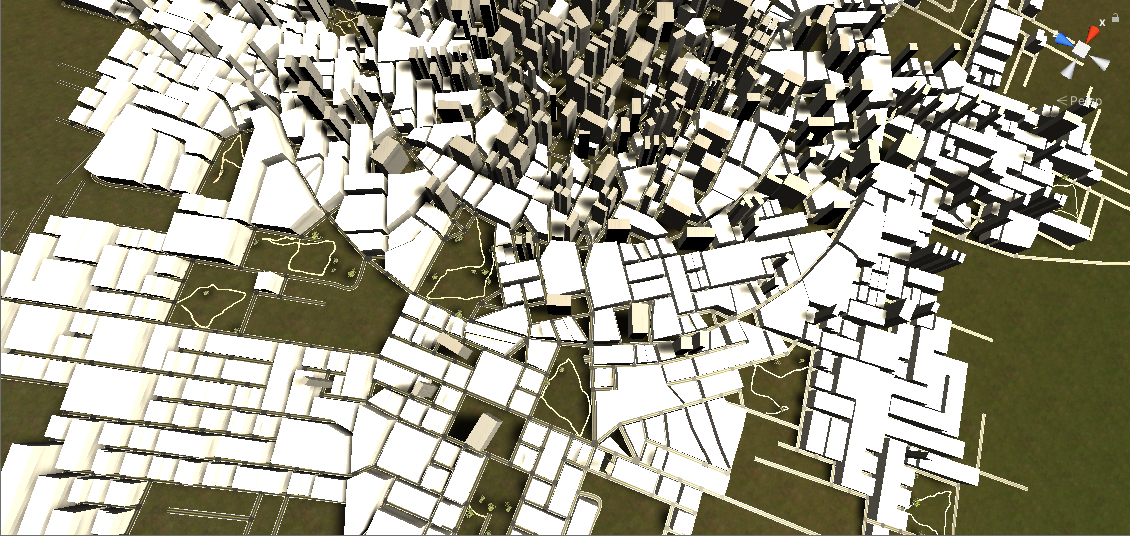
\includegraphics[width=\linewidth]{figure/notforcingloops.png}
 \caption{Example of a generated city filled with parks and buildings.}
 \label{fig:ex}
 \end{figure}
As also visible from Figure~\ref{fig:ex} there are many more generated buildings then there are parks. 
This is actually intentional seeing as the modern cities this project strives to replicate do contain far more buildings than parks. 
The parks are however generated in the largest plots, as it was believed the parks would look best when given a lot of room (see Figure ~\ref{fig:parks}). 

\begin{figure}[H]
   \centering
   \begin{subfigure}[b]{0.4\textwidth}
     \frame{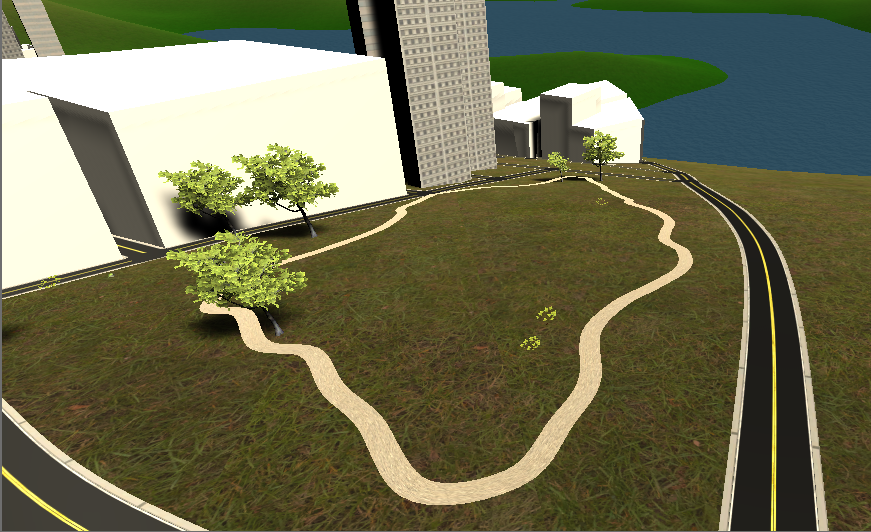
\includegraphics[width=\textwidth]{figure/loopy}}
     \caption{Park with looping path.}
   \end{subfigure}
   \quad
   \begin{subfigure}[b]{0.4\textwidth}
     \frame{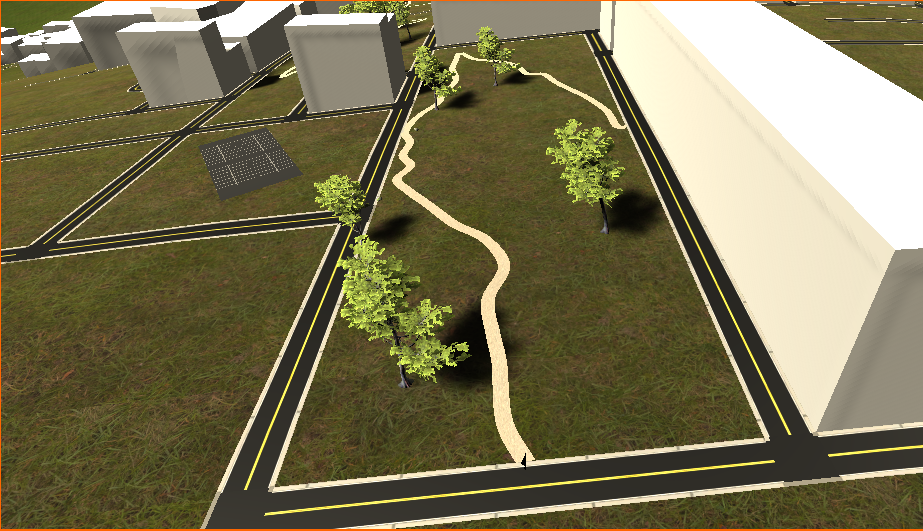
\includegraphics[width=\textwidth]{figure/path}}
     \caption{Park with path that does not loop.}
   \end{subfigure}
   \caption{Two example of different generated parks. One with a path that loops back, and one that creates a path to another edge of the plot.}
   \label{fig:parks}
 \end{figure}
 
 It is worth noting that even though the paths always end up looping, or connecting to a random edge, their shapes still vary a lot, leading to quite interesting results (see Figure~\ref{fig:ex2}).
 The fact that object placement takes the path into consideration also make the park layout appear less random and more relative to its environment. 
 This provides a more consistent feeling to the different parks.
 
 \begin{figure}[H]
   \centering
   \begin{subfigure}[b]{0.4\textwidth}
     \frame{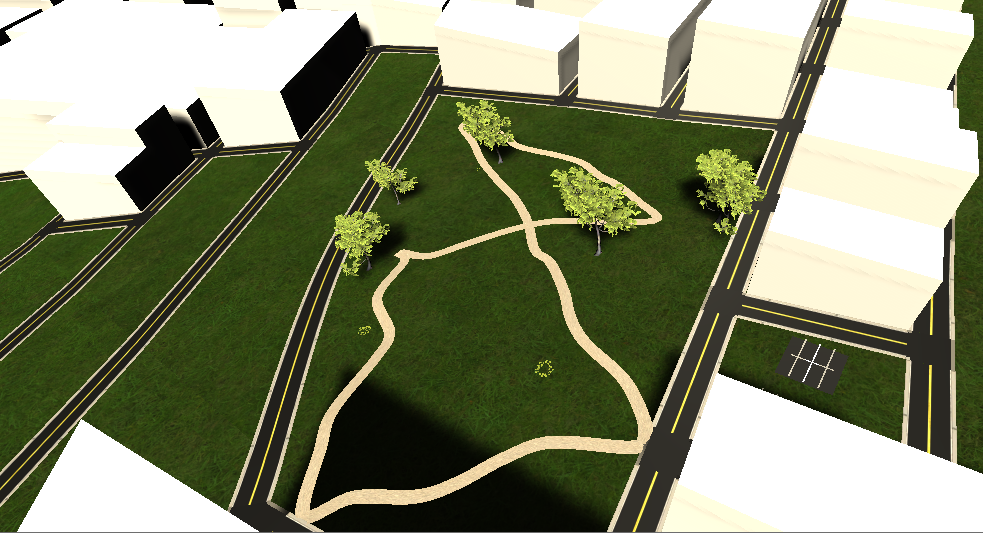
\includegraphics[width=\textwidth]{figure/loopytwo}}
   \end{subfigure}
   \quad
   \begin{subfigure}[b]{0.4\textwidth}
     \frame{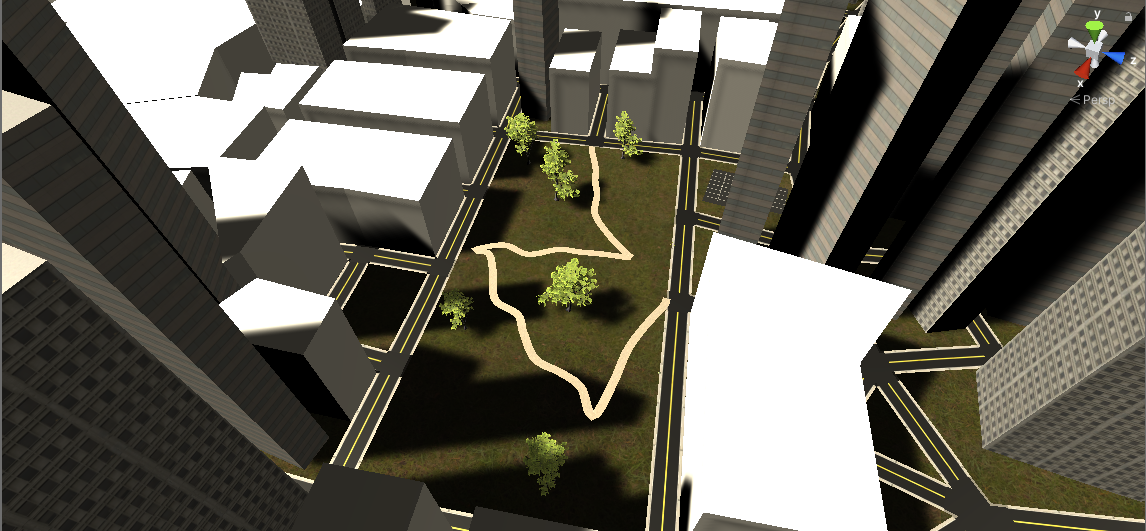
\includegraphics[width=\textwidth]{figure/nonlooptwo}}
   \end{subfigure}
   \caption{Two additional examples, showcasing additional different results.}
   \label{fig:ex2}
 \end{figure}
 
 
 
 

 
 

	